\chapter{Problemanalyse}
\section{Identifikation af problem}
SC-Tronics præsenterer sin nye IoT-løsning \emph{saWux} til en fremlæggelse på ITU, d. 24-08-2020. \emph{saWux} er en datadrevet energi- og klimastyringsløsning, der har til formål at udskifte den konventionelle stikkontakt med alt fra automatiserede stikkontakter og watt-målere til stikkontakter med timere, CO$_2$-målere, temperaturmåling og luftkvalitetsmåling \citep{sawux}.\\

I den sammenhæng stiller SC-T udfordringen, at de søger hjælp til at visualisere den data, som \emph{saWux} indsamler, således at det giver mening og overskueliggøres for deres brugere \citep{virksomhedspresentation}. Problemstillingen er dels at finde en målgruppe og få indsigt i denne — til fordel for både SC-T i fremtiden og ikke mindst for projektet. Desuden beder SC-T om hjælp til den kreative proces, for at skabe den bedste visualisering som muligt og skabe nye idéer til, hvordan man effektivt illustrerer en større mængde data \citep{virksomhedspresentation}.\\

\section{Fremgangsmåde og metoder}
Den første research undersøger, hvordan man effektivt visualiserer data, samt om der eksiterer andre produkter og konkurrenter på markedet, der udbyder det samme som \emph{saWux}. Ved læsning og research af empiri og artikler blev der dannet et grundlag for udarbejdelsen af egen visualisering, som skal eksemplificeres ved hjælp af en mockup og en teknisk beskrivelse.\\

Herefter defineres en målgruppe, som det giver mening at appellere til. Familier med hjemmeboende børn kommer hurtigt på tegnebrættet på baggrund af interesse og tilgængelighed. Under et interview med SC-T gør de selv udtryk for interesse i denne målgruppe.\\

Teorien og empirien udbygges nu på baggrund af målgruppen. En brugerundersøgelse udarbejdes (se bilag \ref{appendix:survey}), som påpeger, at Line Charts — hvor hvert punkt på grafen aflæses med markøren — er et godt grafværktøj til at sammenligne data. Derudover viste undersøgelsen, at der er en indikator, der beskriver den gennemsnitlige værdi ved siden af hver graf (bilag \ref{appendix:survey}). Metoderne, der er blevet brugt, er altså en blanding mellem kilde- og dataresearch samt indsamling af egen data i form af både kvantitative og kvalitative undersøgelser.\\

\section{Målgruppeanalyse}
\cite{osterwalder} fremhæver i teori for “Value Proposition Design”, hvordan virksomheders produkter skal tiltænkes kunden. På den ene side undersøges kundernes profil, mens produktet på den anden side sættes i højsædet, hvilket skaber værdi for kunden.\\

Målgruppen for vores løsning er familier med hjemmeboende børn, med henblik på især at ramme familiens overhoved. Denne målgruppe er interessant, fordi interessen for at spare på kWh-forbruget i husstande stiger \cite[p. 34]{ens.dk}. Familier med hjemmeboende børn er særligt attraktive, da der er tale om et generationsmøde, hvoraf den yngre generation er stærkt klimabevidste \citep{energiwatch}. Flere studier — som for eksempel \cite{gronhoj} — peger på at forældrenes klimahandlinger smitter af på deres børn, og dermed er flere forældre opsatte på at være eksemplariske. \emph{saWux} tilbyder løsningen, der stiller det gode eksempel — og tilmed muliggør \emph{saWux Visualizer}-appen inddragelse af hele familien.

\subsection{Kvantitativt brugerundersøgelse}
I forbindelse med udarbejdelsen af vores visualiseringsapplikation, konstruerer vi en undersøgelse med henblik på at finde den mest brugervenlige visualiseringsværktøj (se bilag \ref{appendix:survey}). Vi når ud til 38 mennesker i alderen 0 til 60. Visualiseringsmetoderne bliver vurderet og rangeret i et pointsystem, der ligger til grundlag for de valgte grafer og udseender i \emph{saWux Visualizer}.

\subsection{Kvalitativt interview}
I forbindelse med udarbejdelsen af vores \emph{Value Proposition Canvas} interviewes et individ fra vores målgruppe (se bilag \ref{appendix:interview}). Interviewet har til formål at opnå en højere indsigt af kundernes “Customer Profile”. Resultatet af interviewet be- og afkræfter flere af de forventninger, der er til kundens jobs, pains og gains. Hermed illustreres kundernes behov gennem “The Value Proposition Canvas” \citep{osterwalder}, hvorfor SC-T’s målgruppe udspecificeres. Illustreret nedenfor i figur \ref{img:problem:canvas}.

\begin{figure}[H]
    \centering
    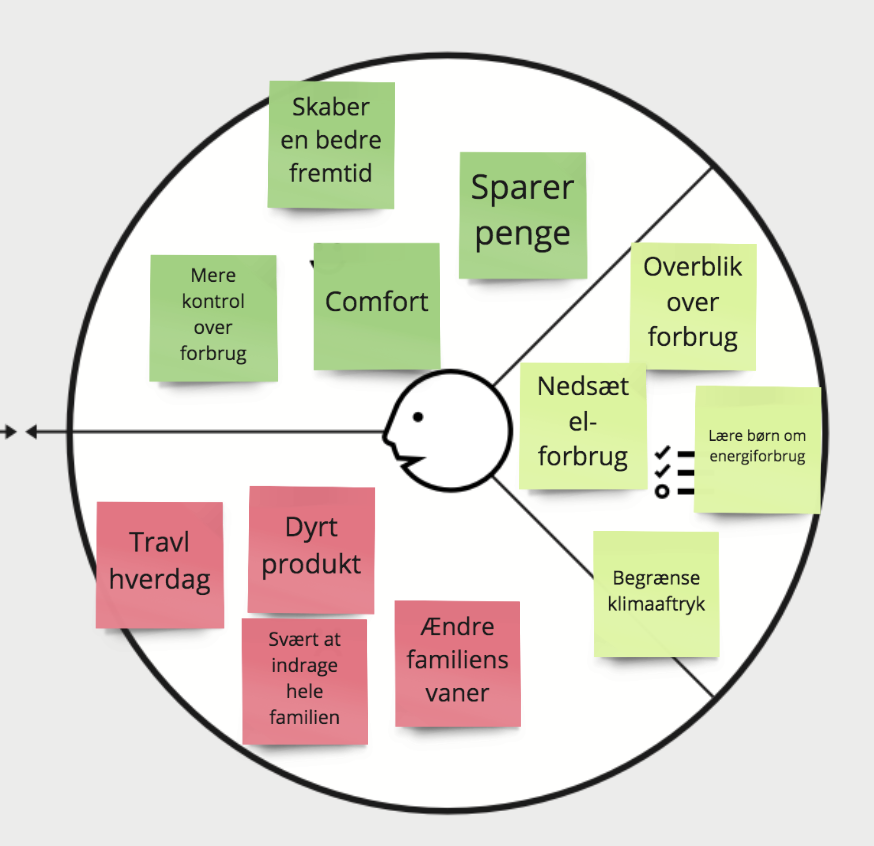
\includegraphics[width=0.5\textwidth]{Images/Value Proposition Design.png}
    \caption[\emph{Value Proposition Canvas}]{\emph{Value Proposition Canvas}, der viser brugerens \emph{jobs, pains} og \emph{gains}}
    \label{img:problem:canvas}
\end{figure}

\section{Resultater til beslutninger}
SC-Tronics fortæller til præsentationen på ITU — og skriver det desuden på \emph{saWux} egen hjemmeside — at de har flere målgrupper, de gerne appellerer til med sit produkt (\cite{virksomhedspresentation} og \cite{sawux}).
Til dels målretter de sig til både private og offentlige virksomheder, og dels til de private forbrugere og “DIY handymen- og girls” \cite{sawux}. SC-Tronics profilerer \emph{saWux} på at være let tilgængelig, billig, intuitiv og mulig at installere selv — uden en autoriseret el-installatør \citep{virksomhedspresentation}. Det er de private forbrugere, dette projekt fokuserer på; det er målgruppen til visualiseringen af \emph{saWux}' data. Mere konkret; familier med hjemmeboende børn. Dette valg er taget for at kunne ramme samspillet mellem to generationer — de energitænkende og  miljøbevidste \citep{energiwatch}. Allerede IT-kompetente og miljøbevidste forældre vil gerne forbedre sine børns liv og give bevidstheden videre til deres børn. \citep{stacey}.\\

Resultatet af de to undersøgelser viser, at denne målgruppe står med et ønske om at spare penge og få et bedre overblik over sit forbrug i en travl hverdag. Målgruppen har en god forståelse af simple grafer med interaktivitet og gennemsnitlige tal (se bilag \ref{appendix:survey}).